\chapter{Opgaveformulering}
Opgaven er at beskrive og udvikle et system, som kan simulere tilstedeværelse i et hjem. 
Dette sker ved at elektriske enheder tændes, slukkes og lignende, når ingen er hjemme. 
Systemet skal indeholde en central transmitter controller (STK500 kit) samt en receiver controller (STK500 kit) med hver sit dertilhørende hardware tilkoblet en elektrisk enhed.
Systemet skal kunne styres og konfigureres vha. en PC og kunne udføre det indstillede scenarie selvom PC’en er slukket. 
Systemet skal desuden indeholde en kodelås (FPGA på DE2 board), som skal være låst op, før det er muligt at tilgå systemets software på PC'en.
Kommunikation mellem controllere skal foregå ved via kommunikation på elnettet. 
Der skal anvendes X.10 protokol\cite[s.12]{lib:AN236} til kommunikationen.
Af sikkerhedsmæssige årsager, skal systemet realiseres på et $18 VAC$ elnet i stedet for det almindelige $230 VAC$. 
\begin{figure}[h]
\centering 
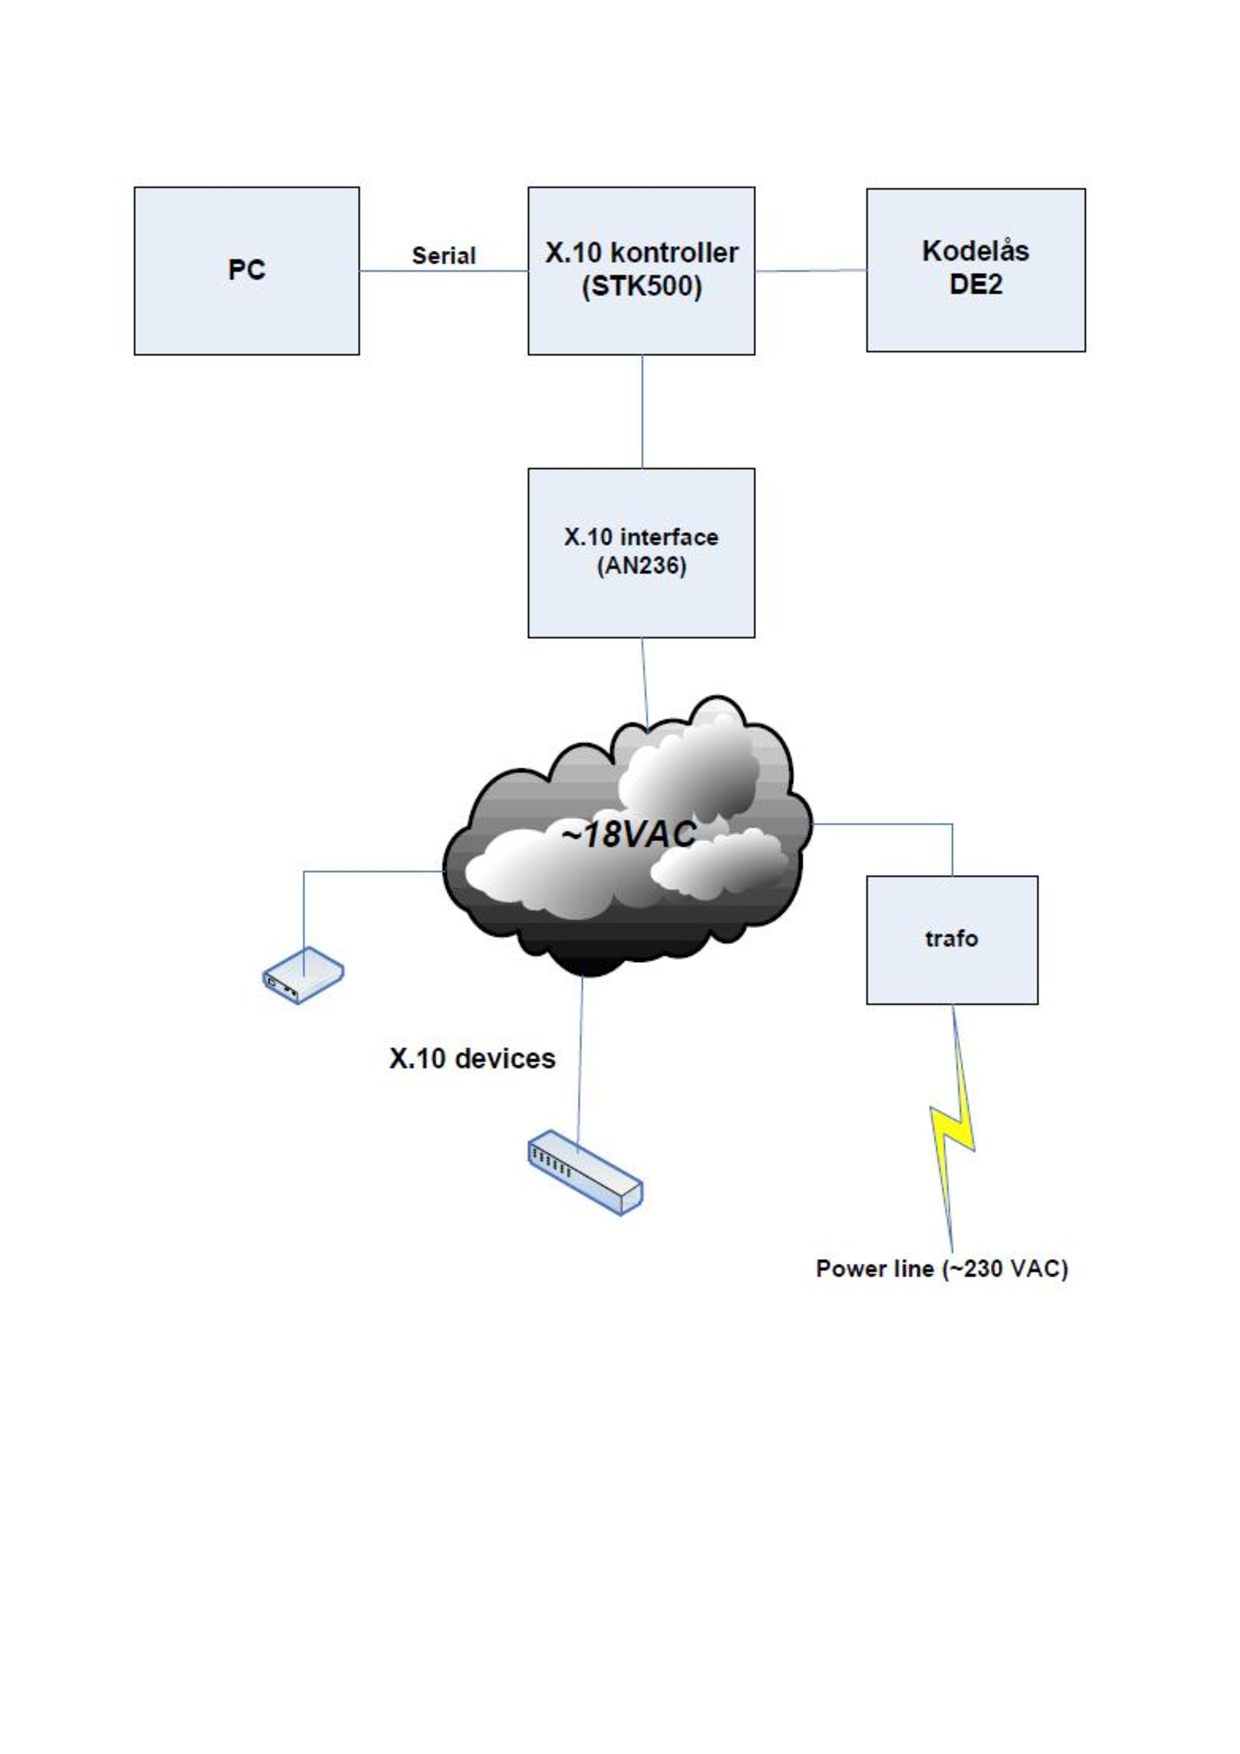
\includegraphics[width={\textwidth-2cm}, trim=0 220 0 50, clip=true] {Opgaveformulering/HW_setup.pdf}
\caption{Home Security System - HW setup \cite[s. 2]{lib:Projektoplaeg}}
\end{figure}

\clearpage